\section{Introduction}



%%%%%%%%%%%%%%%%%%%%%%%%%%%%%%%%%%%%%%%%%
\begin{frame}[fragile]{But ... What is poetry?}

\begin{block}{Definition}
{\small \textbf{Poetry} is a piece of writing or speaking, which
\textbf{\textcolor{red}{MUST}} follow specific
\alert{\underline{\textbf{Patterns}}}.
}\end{block}

%People can easily determine whether a piece of writing is a poem or prose, but ONLY specialists can determine the class of poem.\\

\begin{example}
	\begin{center}
		\begin{Arabic}
			%@@@change this Bayt
			وُلِـدَ الـهُـدى فَـالكائِناتُ ضِياءُ\hspace{3em}  وَفَـمُ الـزَمـانِ تَـبَـسُّـمٌ وَثَناءُ
		\end{Arabic}
	\end{center}
\end{example}

\end{frame}

%%%%%%%%%%%%%%%%%%%%%%%%%%%%%%%%%%%%%%%%%
\begin{frame}[fragile]{Arabic Prosody \textarabic{العَرُوض}}
\begin{columns}
\begin{column}{0.6\textwidth}
	\textit{Al-Farahidi} (718 – 786 CE) analyzed the Arabic poetry, then he discovered the \alert{\underline{\textbf{Patterns}}} which is the succession of consonants and vowels.
\end{column}
\begin{column}{0.4\textwidth}
		\begin{figure}
			\begin{center}
				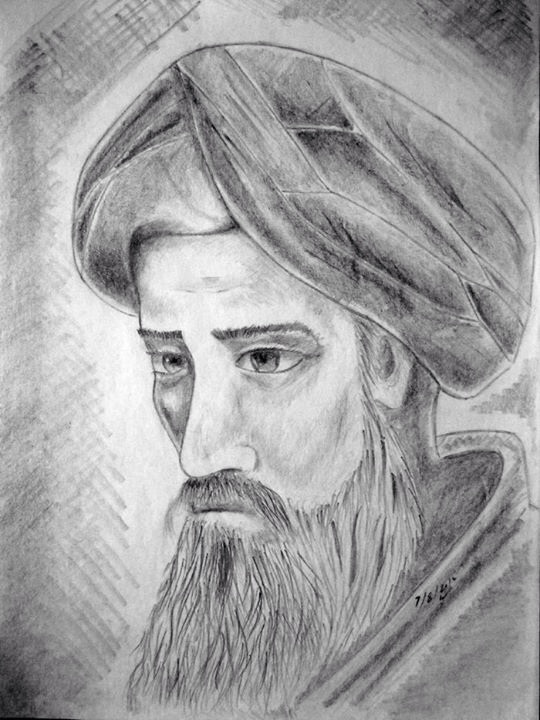
\includegraphics[width=0.6\textwidth]{Figures/Al-Farahidi.jpg}
				\caption{\textit{Al-Farahidi}\\
{\tiny figure taken from \url{https://goo.gl/ZJySa8}}.}
			\end{center}
		\end{figure}
\end{column}
\end{columns}
\end{frame}

%%%%%%%%%%%%%%%%%%%%%%%%%%%%%%%%%%%%%%%%%
\begin{frame}[fragile]{Arabic Prosody \textarabic{العَرُوض}}

\begin{itemize}
	\item<1-> A \textbf{poem } is a set of verses having the same meter and rhyme.
	\item<2-> \textbf{Vowels}  carry one of \textarabic{◌َ  ◌ُ  ◌ِ} which represent the following short vowels /a/, /u/, /i/.
	\item<3-> \textbf{Consonants} carry \textarabic{◌ْ}.
	\item<4-> \textbf{Shadaa} indicates the letter is doubled \textarabic{◌ّ}. 
	\item<5-> \textbf{Tanween} \textit{harakah} and \textit{Noon} letter with consonant to the end of the word. It sounds /n/.
\end{itemize}

\end{frame}
%%%%%%%%%%%%%%%%%%%%%%%%%%%%%%%%%%%%%%%%%%%%%%


%%%%%%%%%%%%%%%%%%%%%%%%%%%%%%%%%%%%%%%%%
\begin{frame}[fragile]{Arabic Prosody \textarabic{العَرُوض}}
\begin{columns}
	
	\begin{column}{.7\textwidth} % Left column and width
		{\small 	
		- A \textbf{foot}(\textit{tafa'ilah} \textarabic{التفعيلة}) : is an \textbf{ordered} sequence of vowels and consonants. \\
		- \textbf{Meter} \textarabic{البحر}: is an \textbf{ordered} sequence of \alert{feet}. }

		\begin{table}
		\small
				\begin{tabular}[h!]{|c|c|} 
			\hline
			\textbf{Meter Name} & \textbf{Meter} \small{\textit{feet combination}} \\ 
			\hline
			\textit{\alert{al-Wafeer}}    & \textarabic{مُفَاعَلَتُن مُفَاعَلَتُن مُفَاْعَلْ} \\ %
			\textit{al-Taweel}    & \textarabic{فَعُوْلُنْ مَفَاْعِيْلُنْ فَعُوْلُنْ مَفَاْعِلُنْ} \\ %
			\vdots                &  \vdots\\
			\textit{al-Moktadib}  & \textarabic{مَفْعُوْلاتُ مُسْتَفْعِلُنْ مُسْتَفْعِلُن} \\
			\textit{al-Modar'e}   & \textarabic{مَفَاْعِيْلُنْ فَاْعِلاتُنْ مَفَاْعِيْلُنْ} \\
			\hline
		\end{tabular}
		\end{table}
	\end{column}%
		\hfill%
		\begin{column}{.3 \textwidth}
			\begin{table}
				\small
			\begin{tabular}{|c|c|} \hline
			\textbf{Feet} & \textbf{Scansion} \\
			\hline
			\textarabic{فَعُولُنْ}  & \texttt{0/0//}\\
			\textarabic{فَاعِلُنْ}  & \texttt{0//0/}\\
			\textarabic{مُسْتَفْعِلُنْ}& \texttt{0//0/0/}\\
			\textarabic{مَفاعِيلُنْ}& \texttt{0/0/0//}\\
			\textarabic{مَفْعُولاَت} & \texttt{0//0///}\\
			\textarabic{فَاعِلاَتُنْ} & \texttt{0/0//0/}\\
			\textarabic{مُفَاعَلَتُنْ}& \texttt{0///0//}\\
			\textarabic{مُتَفَاعِلُنْ}& \texttt{0//0///}\\
			\hline
		\end{tabular}
		\end{table}		

	\end{column}
\end{columns}
\begin{center}
	\begin{Arabic}
		\begin{table}
			\small
			\begin{tabular}[h!]{c c c c c c} 
%				\hline
				\multicolumn{3}{c} \hfil \textarabic{ إِذَا لَــمْ تَـخْــشَ عَـاقِـبَـةَ اللَّـيـالِـي}  \hfil  & \multicolumn{3}{c} \hfil \textarabic{وَلَـمْ تَـسْـتَـحْـيِ فَـاصْنَـعْ مَـا تَـشَـاءُ} \hfil \\ 
				{\color{purple} \textarabic{إِذَا لَمْ تَخْـ}} & {\color{blue} \textarabic{ ـشَ عَاقِبَةَ لـْ}}& {\color{OliveGreen}\textarabic{ ـلَيالِيْ}} & 
				{\color{purple}\textarabic{ وَلَمْ تَسْتَحـْ}} &{\color{blue} \textarabic{ ـيِ فَصْنَعْ مَا}} &{\color{OliveGreen}\textarabic{ تَشَاءُوْ}}\\
				{\color{purple} \texttt{//0/0/0}} & {\color{blue} \texttt{//0/0/0}} & {\color{OliveGreen} \texttt{//0/0}} &
				{\color{purple} \texttt{//0/0/0}} & {\color{blue} \texttt{//0/0/0}} & {\color{OliveGreen} \texttt{//0/0}}\\
				{\color{purple} \textarabic{مُفَاْعَلْتُنْ}} &{\color{blue}\textarabic{ مُفَاْعَلْتُنْ}} &{\color{OliveGreen} \textarabic{مُفَاْعَلْ}}&
				{\color{purple}\textarabic{مُفَاْعَلْتُنْ}}& {\color{blue}\textarabic{ مُفَاْعَلْتُنْ}}& {\color{OliveGreen}\textarabic{ مُفَاْعَلْ}}\\
%				\hline
			\end{tabular}
		\end{table}
	\end{Arabic}%
	
\end{center}


\end{frame}

%%%%%%%%%%%%%%%%%%%%%%%%%%%%%%%%%%%%%%%%%%%%%%%%%%%%%%%%%%%%%

%%%%%%%%%%%%%%%%%%%%%%%%%%%%%%%%%%%%%%%%%
\begin{frame}
\frametitle{Thesis Working Steps.}
\begin{figure}[!t]
	   \begin{tikzpicture}[>=latex']
        \tikzset{block/.style= {draw, rectangle, align=center,minimum width=2cm,minimum height=1cm},
        rblock/.style={draw, shape=rectangle,rounded corners=1.5em,align=center,minimum width=2cm,minimum height=1cm},
        input/.style={ % requires library shapes.geometric
        draw,
        trapezium,
        trapezium left angle=60,
        trapezium right angle=120,
        minimum width=2cm,
        align=center,
        minimum height=1cm
    },
        }
        \node [rblock]  (start) {Start};
        \node [block, right =1cm of start] (crawl) {Data Crawling};
        \node [block, right =1cm of crawl] (clean) {Data Cleansing};
        \node [block, right =1cm of clean] (encode) {Data Encoding};
        \node [block, below right =2cm and -0.5cm of start] (train) {Training};
        \node [block, right =1cm of train] (validate) {Validation \& Testing};
        \node [block, right =1cm of validate] (choose) {select Best Model};
        \node [rblock, right =1cm of choose] (end) {End};
        \node [coordinate, below right =1cm and 1cm of encode] (right) {};  %% Coordinate on right and middle
        \node [coordinate,above left =1cm and 1cm of train] (left) {};  %% Coordinate on left and middle
        \node [coordinate,below  =1cm and 1cm of validate] (loop) {};  %% Coordinate on left and middle

%% paths
        \path[draw,->] (start) edge (crawl)
                    (crawl) edge (clean)
                    (clean) edge (encode)
                    (encode.east) -| (right) -- (left) |- (train)
                    (train) edge (validate)
                    (validate) -- (loop) -| (train)
                    (validate) edge (choose)
                    (choose) edge (end)
                    ;
    \end{tikzpicture}

%%% Local Variables:
%%% mode: latex
%%% TeX-master: t
%%% End:

	\caption{Thesis Working Steps.}
	\label{Fig:Thesis_Cycle}
\end{figure}

\end{frame}
%%%%%%%%%%%%%%%%%%%%%%%%%%%%%%%%%%%%%%%%%
%
%\begin{frame}
%\frametitle{Sample frame title}
%This is a text in second frame. For the sake of showing an example.
%
%\begin{itemize}
%    \item<1-> Text visible on slide 1
%    \item<2-> Text visible on slide 2
%    \item<3-> Text visible on slide 3
%    \item<4-> Text visible on slide 4
%\end{itemize}
%\end{frame}
%
%%%---------------------------------------------------------
%%%Example of the \pause command
%\begin{frame}
%In this slide \pause
%
%the text will be partially visible \pause
%
%And finally everything will be there
%\end{frame}
%
%\section{Second section}
%
%%%---------------------------------------------------------
%%%Highlighting text
%\begin{frame}
%\frametitle{Sample frame title}
%
%In this slide, some important text will be
%\alert{highlighted} beause it's important.
%Please, don't abuse it.
%
%\begin{block}{Remark}
%Sample text
%\end{block}
%
%\begin{alertblock}{Important theorem}
%Sample text in red box
%\end{alertblock}
%

%\end{frame}
%%%---------------------------------------------------------
%%
%%
%%%---------------------------------------------------------
%%%Two columns
%\begin{frame}
%\frametitle{Two-column slide}
%
%\begin{columns}
%
%\column{0.5\textwidth}
%This is a text in first column.
%$$E=mc^2$$
%\begin{itemize}
%\item First item
%\item Second item
%\end{itemize}
%
%\column{0.5\textwidth}
%This text will be in the second column
%and on a second tought this is a nice looking
%layout in some cases.
%\end{columns}
%\end{frame}
%%---------------------------------------------------------



%%%%%%%%%%%%%%%%%%%%%%%%%%%%%%%%%%%%%%%%%%%%%%%%%%%%%%%%%%%%%%%%%%%%%%%%%%%
%%% Local Variables:
%%% mode: latex
%%% TeX-master: "../main"
%%% TeX-engine: xetex
%%% End:
